% label prefix for this part: dat
\chapter{Project dat}\label{sec:dat}

\section{Einführung}

In der heutigen Gesellschaft wird der Austausch von Daten immer wichtiger. Vermehrt werden grosse Datenmengen unterschiedlichster Art - aus Forschung, Regierung oder zivilen Kreisen - zur allgemeinen Verwendung angeboten. Nicht nur die Art der Daten ist jedoch vielfältig, sondern auch Datenformat oder Zugriffsart unterscheiden sich.

Das \gls{dat}-Projekt hat das Ziel, die Integration sowie einen einheitlichen Zugriff solcher Datenquellen vereinfachen.

Als erstes Ziel dieser Arbeit sollte das noch junge Projekt \gls{dat} anlysiert und dessen genaue Funktionalität und Funktionsweise dokumentiert werden. Aufgrund der Tatsache, dass \gls{dat} noch relativ neu ist und sich in der Alphaphase befindet, ist das Projekt nur wenig und sehr verstreut dokumentiert. \Gls{dat} hat im Jahr 2014 einen Gesamtbetrag von \SI{310000}[{\$}]{} von der \gls{knight-foundation} sowie der \gls{sloan-foundation} zur Weiterentwicklung des Projekts erhalten, was als Indiz für ein vielversprechendes Projekt gilt.

\section{Was ist dat?} % https://github.com/maxogden/dat/blob/master/docs/what-is-dat.md

Das dat-Projekt hat folgende Ziele\cite{what-is-dat}: 

\begin{itemize}
\item Daten sollen automatisch zwischen unterschiedlichen dat-Instanzen synchronisiert werden können. 
\item Unterstützung grosser Datenmengen\footnote{Milliarden von Datensätzen bzw. Speicherbedarf im \si{\tera\byte}-Bereich}, evtl. mit häufigen Aktualisierungen
\item Unterstützung von tabellarischen oder unstrukturierten Daten
\item Plugin-basierte Schnittstelle zu bestehenden Datenbanken/Formaten
\item Unterstützung für automatisierte Workflows
\end{itemize}

% https://github.com/maxogden/dat/blob/master/docs/js-api.md#transformations
Für den Umgang mit verschiedenen Datenformaten können Transformationen\cite[transformations]{dat-js-api} definiert werden, welche entweder vor Schreib- oder nach Lese-Operationen ausgeführt werden.

\section{Architektur}
% diagramm, requirements, interfaces, ...

% http://dat-data.com/docs.html: "Q:If I have multiple different tables that I want to store, would I create a separate dat repo for each? Can a single dat repo store multiple tables? A: Each dat repo is only one table."

dat speichert Daten auf zwei verschiedene Arten:
\begin{itemize}
\item Für Tabellen-Daten wird LevelDB verwendet. Da LevelDB ein austauschbares Backend hat können diese Daten auch in einer SQL-Datenbank wie Postgres gespeichert werden.
\item BLOB-Daten werden standardmässig im File-System per local-blob-store gespeichert. Dies kann ebenfalls durch eine kompatible Implementation ausgetauscht werden.
\end{itemize}

\begin{figure}[H]
  \centering
  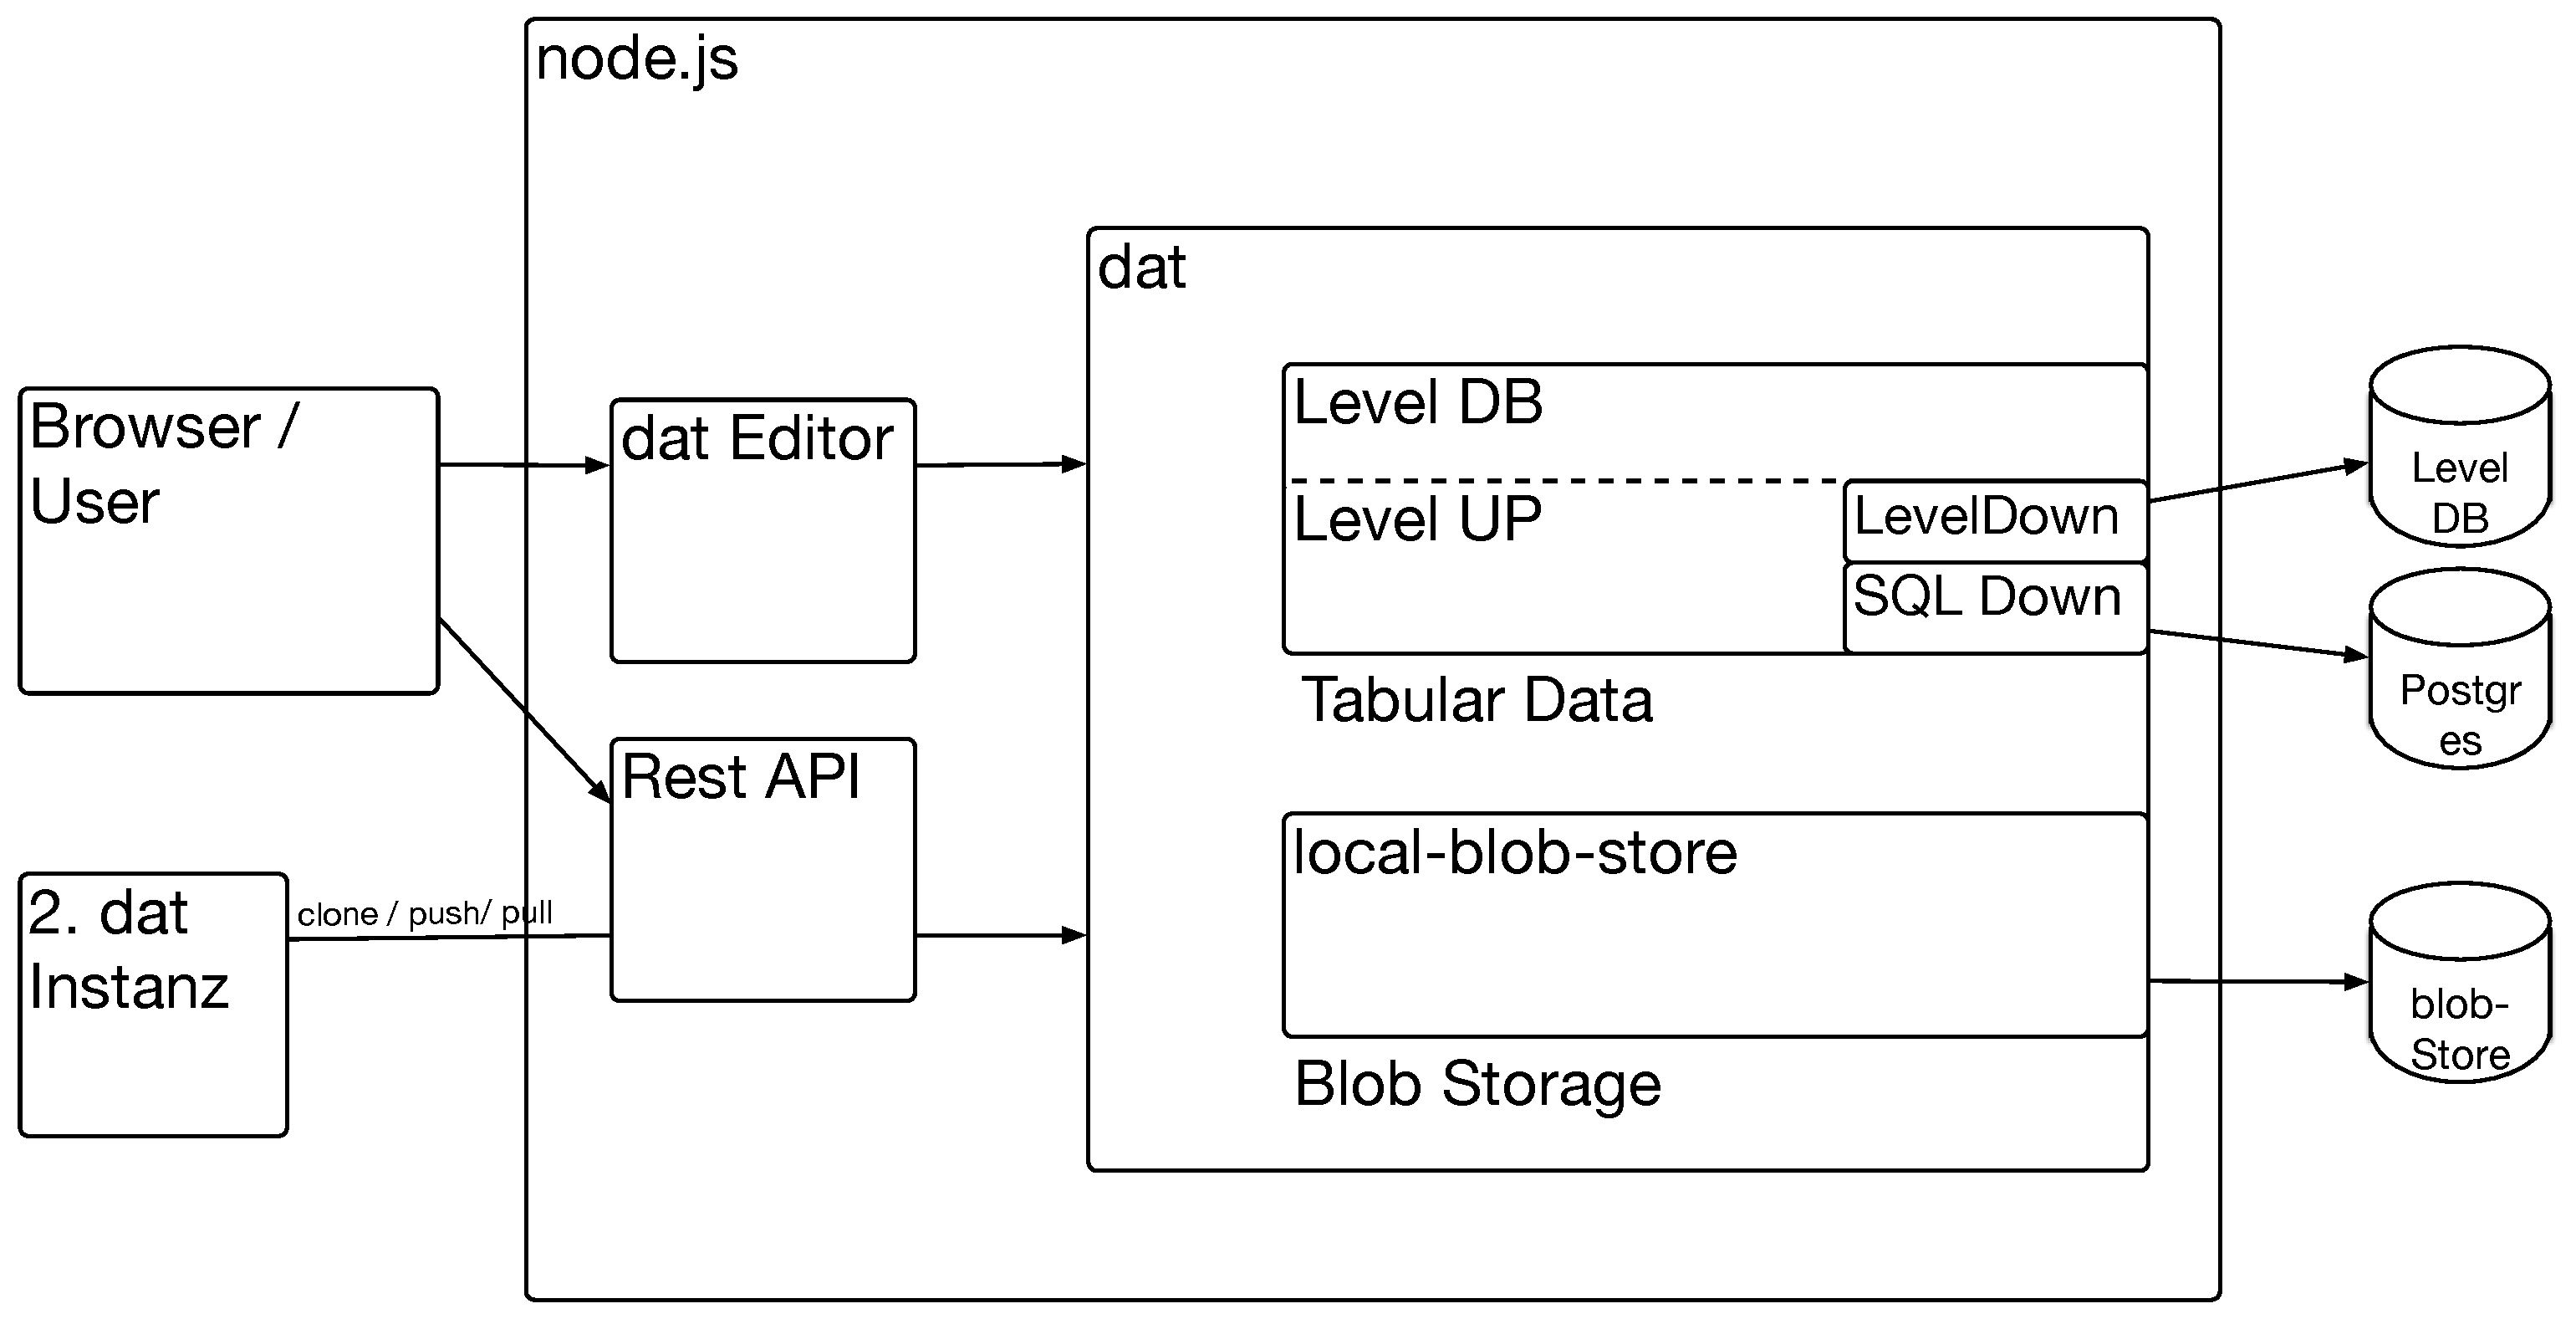
\includegraphics[width=\linewidth,clip]{fig/dat-architecture}
  \caption{dat Architektur-Übersicht}
  \label{fig:dat-architecture-overview}
\end{figure}

Direkt mit dat wird auch der dat-editor geliefert, welcher als rudimentäres Web-GUI dient. Der Editor sowie das REST-API werden gestartet, wenn \mintinline{console}{dat listen} aufgerufen wird. Andere dat-Instanzen verwenden das REST-API für die Synchronisation.
\begin{figure}[H]
  \centering
  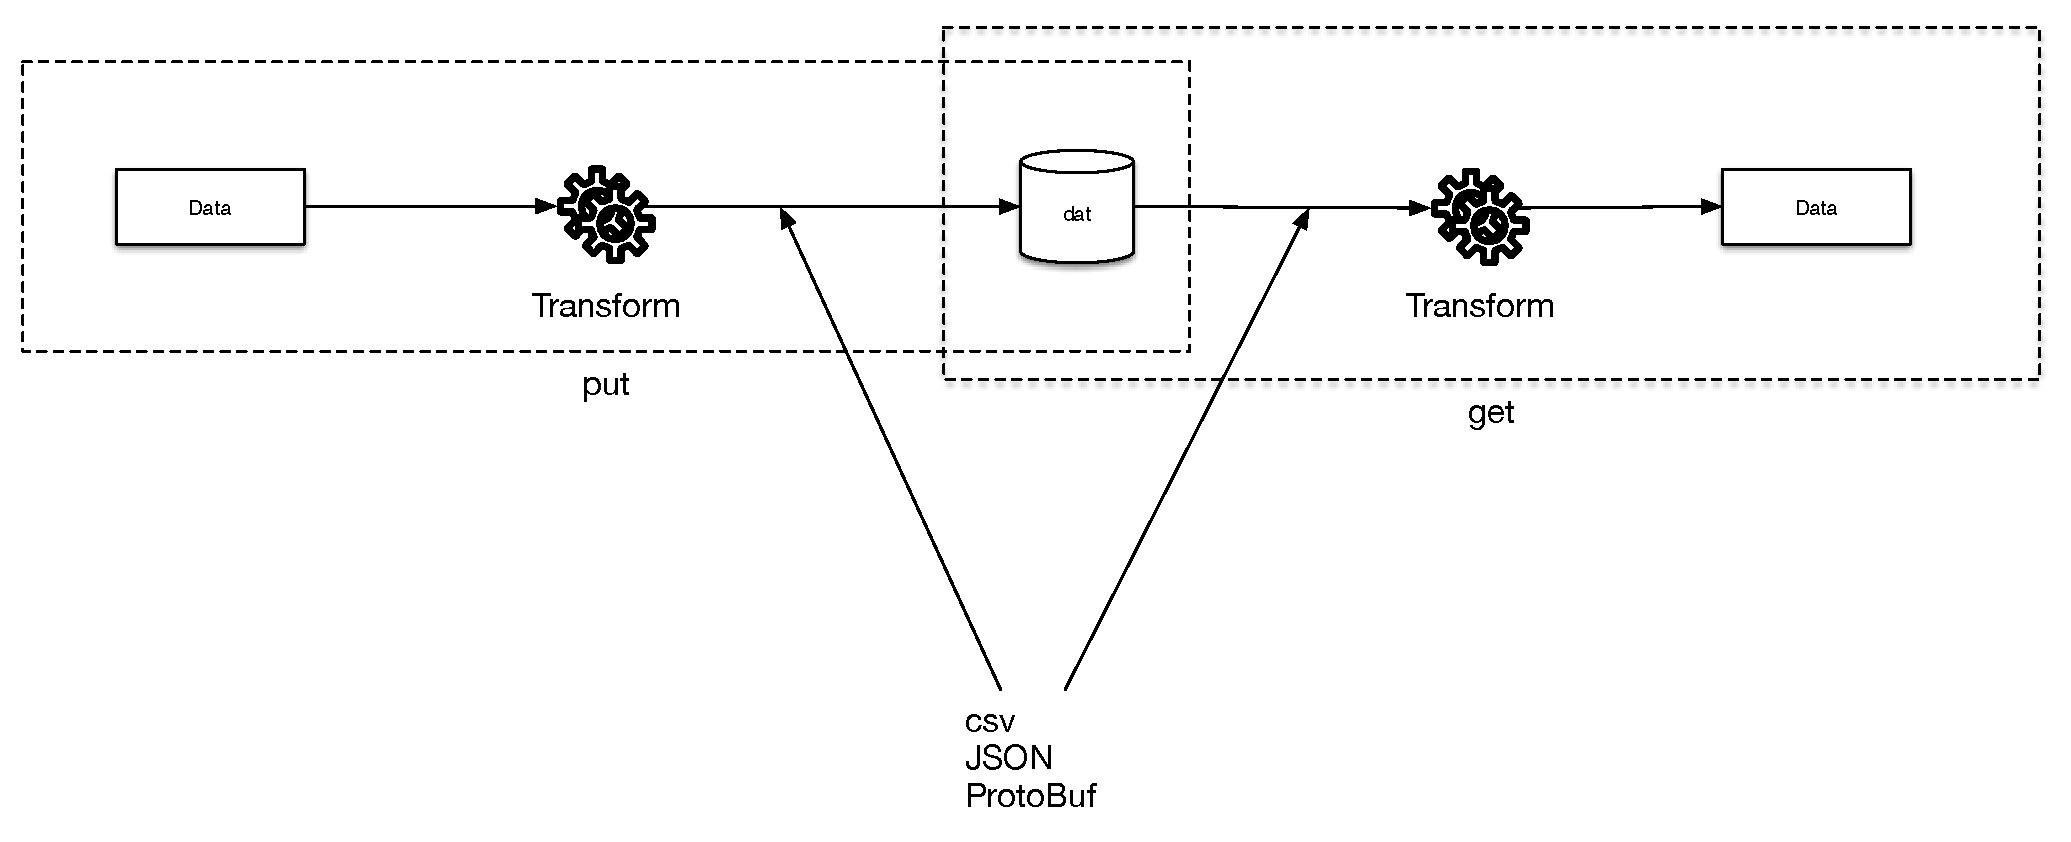
\includegraphics[width=\linewidth,clip]{fig/dat-pipeline}
  \caption{dat Daten-Pipelines}
  \label{fig:dat-architecture-pipeline}
\end{figure}

Mithilfe des Sub-Projekts \texttt{gasket} können sogenannte Daten-Pipelines definiert werden. Diese dienen dazu, Daten abzurufen, zu transformieren und schliesslich in dat zu speichern, bzw. Daten aus dat zu lesen, zu transformieren und schliesslich abzuliefern.

\section{Use Cases}
In diesem Abschnitt werden mögliche Verwendungszwecke von \gls{dat} aufgezeigt.

\subsection{Astronomie \textendash\ Trillian} 
% https://github.com/maxogden/dat/issues/172
% https://github.com/trillian/trillian
% http://trillianverse.com (nicht verfügbar 2015-02-23)
In der Astronomie fallen riesige Datenmengen an. Teilweise werden diese als grosse Daten-Releases zur Verfügung gestellt (z.B. Sloan Digital Sky Survey), welche frühere Releases komplett ersetzen. Andere Projekte stellen inkrementelle Updates zur Verfügung (z.B. Hubble). Viele Astronomie-Institute haben weder die Mittel noch das Know-how, mit solchen Datenmengen umgehen zu können. Das Trillian-Projekt kümmert sich um die Verwaltung dieser Daten und bietet eine Compute-Engine an, um neue Modelle anhand der vorhandenen Daten zu testen.

dat soll für den Import und die Indexierung der Daten verwendet werden.

Siehe auch \url{https://github.com/maxogden/dat/issues/172}.

\subsection{Regierung \textendash\ Sammlung von Daten} % https://github.com/maxogden/dat/issues/153
Für Statistik- oder Regulierungszwecke sammeln Regierungen Daten von unterschiedlichsten Betrieben. Diese Daten müssen oft über ein mehr oder weniger brauchbares Portal abgeliefert werden.

Die Verwendung von dat bringt folgende Vorteile:
\begin{itemize}
\item Ermöglicht die Prüfung von Daten beim Import, bereits vor der Ablieferung der Daten
\item Ermöglicht Ergänzung oder Korrektur von bereits abgelieferten Daten.
\item Ersatz der bisher verwendeten, für jede Regierungsstelle neu kreierten und teuren Portale durch eine standardisierte Lösung.
\end{itemize}

Siehe auch \url{https://github.com/maxogden/dat/issues/153}.

\section{CLI}

%https://github.com/maxogden/dat/blob/master/docs/cli-usage.md

Das \gls{dat} \gls{cli} ``\texttt{dat}'' ist das einzige Werkzeug um ohne API mit dem Repository zu interagieren und bietet folgende Basisfunktionalität:

\begin{itemize}
  \item Erstellung neuer dat Repositories/Intanzen mit \mintinline{console}{$ dat init}
  \item Import von CSV oder JSON Dateien mit \mintinline{console}{$ dat import}
  \item \gls{dat} Server und Webfrontend starten mit \mintinline{console}{$ dat listen}
  \item Klonen eines kompletten\footnote{Samt aller Historie} remote Repositories \gls{dat} Repostitories analog Git mit \mintinline{console}{$ dat clone}
  \item Lokale Änderungen ebenfalls analog Git wieder zurück ins remote Repository synchronisieren mit \mintinline{console}{$ dat push}
  \item Rudimentäre Manipulation und Ausgabe von einzelnen Zeilen des Repositories mit \mintinline{console}{$ dat rows} bzw. \mintinline{console}{$ dat cat}
\end{itemize}

Die abschliessende Liste von zurzeit unterstützten Befehlen ist in 
\vref{app:dat-help} zu finden. Für fortgeschrittenere Verwendung ist das \gls{cli} jedoch nicht geeignet, da viele Optionen fehlen. Stattdessen sollte das JavaScript-API verwendet werden.

Spätere Versionen sollen auch Branches erlauben sowie mit Änderungskonflikten umgehen können.

\section{Frontend}

\Gls{dat} bietet ein minimales Webfrontend welches ähnliche Operationen wie mit dem \gls{cli} wie z.B. Import/Export sowie betrachten der Datensätze ermöglicht. Einen Ausschnitt ist folgender \cref{fig:dat:webfrontend} zu sehen.

\begin{figure}[H]
  \centering
  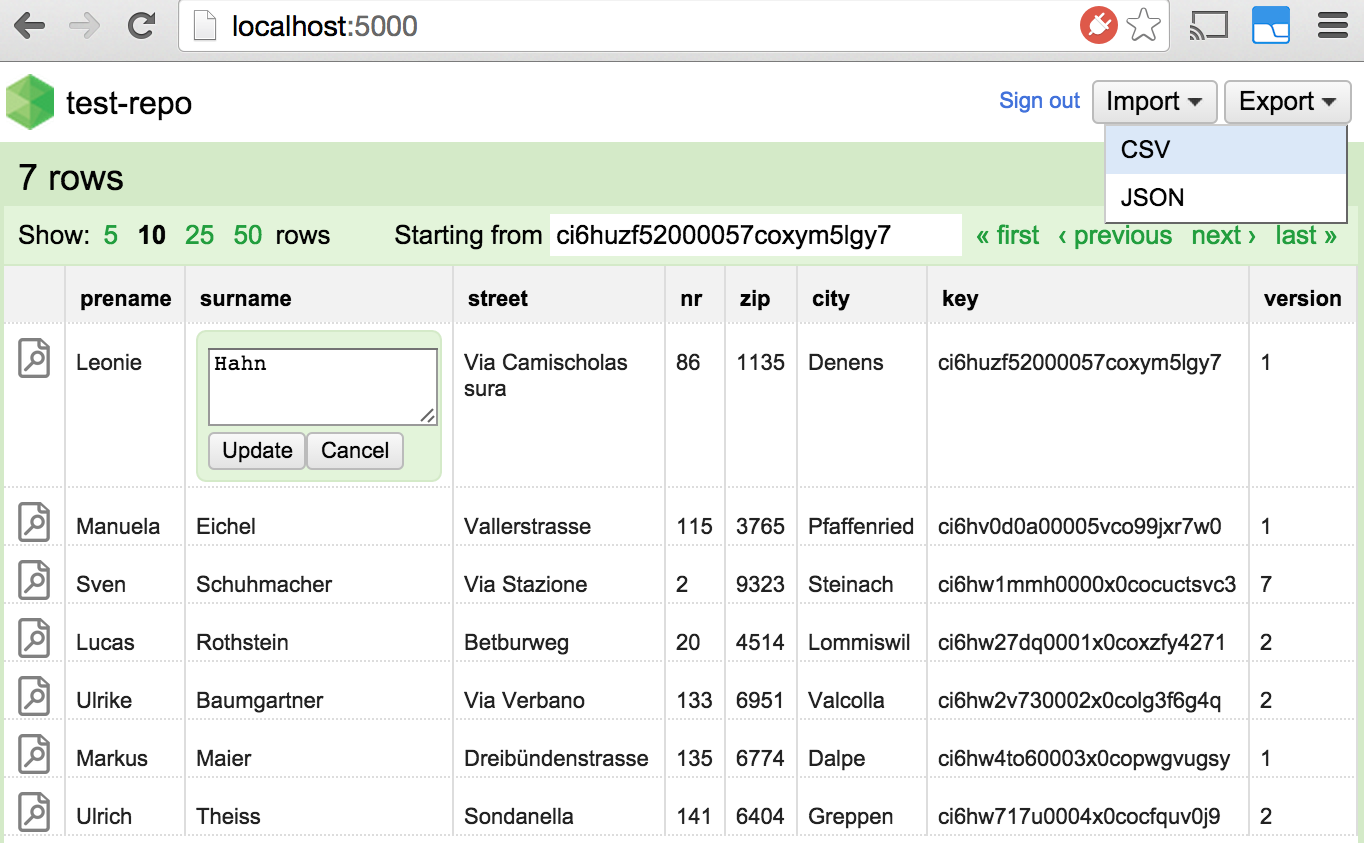
\includegraphics[width=0.8\textwidth]{fig/webfrontend}
  \caption{dat Webfrontend}
  \label{fig:dat:webfrontend}
\end{figure}

\section{Schnittstellen}
Für eine Beschreibung der von \gls{dat} zur Verfügung gestellten \gls{api}, siehe \vref{app:dat}.


\section{Fazit}
%\section{Verwendung}
Zum aktuellen Zeitpunkt (Februar 2015) implementiert dat alpha 6.9.6 folgende Features:
\begin{itemize}
\item Datenspeicher auf Basis eines Key-/Value-Stores (LevelDB).
\item Limitierte Synchronisation basierend auf einem Change-Stream. So weit wir erkennen können ist keine Konflikt-Verwaltung vorhanden, sondern lediglich Ein-Weg-Synchronisation vorgesehen.
\item Pro dat-Instanz existiert nur ein Schema. Falls ein Datensatz mit neuen Spalten hinzugefügt werden soll wird das bereits vorhandene Schema mit dem Schema des neuen Datensatzes zusammengeführt.
\end{itemize}

Aktuell läuft die Entwicklung der dat beta-Version. In dieser sollen mehrere ``datasets'' unterstützt sowie bessere Versionskontrolle mit Konfliktbehandlung bzw. -Vermeidung implementiert werden. Leider ist diese Version noch nicht stabil und das API ändert sich damit komplett.

\begin{decision}[label=dec:dat:fazit]{Projekt dat}
Aufgrund der Tatsache, dass \gls{dat}, obschon vielversprechend, noch sehr unausgereift und undokumentiert ist, sowie das API noch ständigen Änderungen unterzogen wird, wurde nach Rücksprache mit dem Betreuer gegen den Einsatz von \gls{dat} entschieden. Das Projektrisiko ist zu gross und es wird nach einer alternativen Lösungen zur Implementation eines Datenhubs gesucht.
\end{decision}

